\chapter{Stato dell'arte e lavori correlati}\label{cha:stato_dell_arte_e_lavori_correlati}

Durante la definizione del problema (capitolo~\ref{sec:definizione_del_problema}) abbiamo evidenziato come il presente lavoro affronti uno specifico sottoproblema riconducibile ad uno dei più noti problemi NP-hard~\cite{karp1972}, senza tuttavia approfondire effettivamente la definizione formale né le motivazioni che ne giustificano l'interesse.
All'interno del seguente capitolo dunque tratteremo in modo più rigoroso l'introduzione formale al problema nelle sue varianti principali, analizzandone la complessità computazionale e tracciando l'evoluzione dello stato dell'arte: dai modelli statici tradizionali fino alle moderne formulazioni online su flussi di dati, che costituiranno il riferimento per gli sviluppi successivi dell'elaborato.

% 2.1
% Revisione Ready
% Grammatica Ready
% Citazioni Ready

\section{Il problema dell'Hitting Set}\label{sec:il_problema_dell_hitting_set}

Il problema dell'Hitting Set è uno dei pilastri dell'ottimizzazione combinatoria e della teoria della complessità computazionale, noto storicamente per essere uno dei 21 problemi NP-completi di Karp~\cite{karp1972}.
Tale problema riveste una particolare importanza pratica in quanto trova numerose applicazioni in contesti dell'informatica, bioinformatica, data mining e all'interno dei sistemi di diagnostica~\cite{moreno2013, mcguire2014}.
Dal punto di vista teorico, il problema dell'Hitting Set è strettamente correlato al problema noto come \textit{Set Cover}, di cui rappresenta il duale.
Per tale motivo, alcune soluzioni proposte per il Set Cover verranno citate in seguito nell'ambito dei lavori correlati.

\subsection{Definizione formale e varianti}

Sia $U$ un insieme finito, detto universo, e sia $S = \{S_1,S_2,\dots,S_m\}$ una famiglia di sottoinsiemi di U.
Un sottoinsieme $H \subseteq U$ è definito \textit{Hitting Set} per $S$ se interseca ogni sottoinsieme appartenente a $S$, ovvero se
\[
    \forall S_i \in S,\space H \cap S_i \neq \emptyset.
\]
In altre parole, ogni sottoinsieme della collezione, nel nostro caso dunque ogni iperarco, deve contenere almeno un elemento appartenente ad $H$~\cite{garey1979, bretto2013}.
La condizione che rende però tale problema computazionalmente complesso da risolvere non risiede nella difficoltà che si può incontrare nel trovare uno di questi sottoinsiemi, bensì in quella di trovare il sottoinsieme con cardinalità minima che rispetti le proprietà precedentemente citate.

\begin{figure}[h]
    \centering
    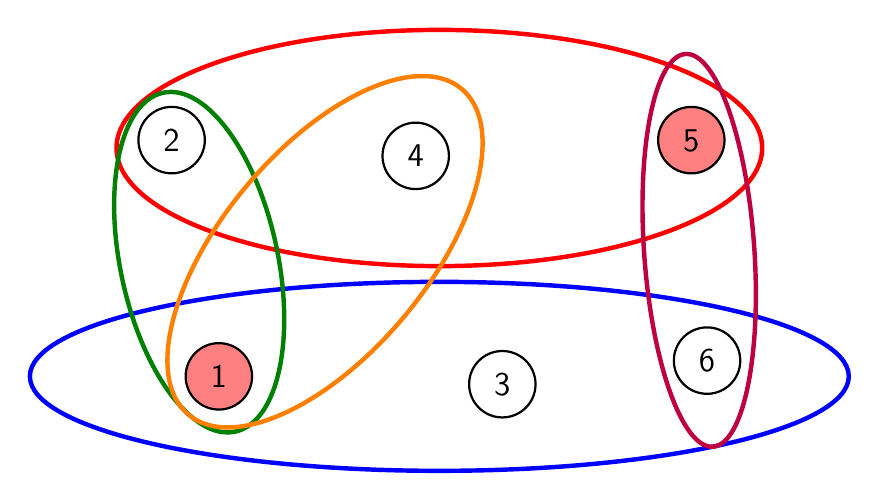
\begin{tikzpicture}[
        % Stile per i nodi standard (bianchi)
        element/.style={circle, draw=black, fill=white, font=\large\sffamily, minimum size=24pt, inner sep=0pt, thick},
        % Stile per i nodi selezionati nel hitting set (rossi)
        hit/.style={element, fill=red!50}
    ]

        % --- COORDINATE DEI NODI ---
        \node[hit]     (N1) at (0.9, 0.2) {1};
        \node[element] (N2) at (0.3, 3.2) {2};
        \node[element] (N3) at (4.5, 0.1) {3};
        \node[element] (N4) at (3.4, 3) {4};
        \node[hit]     (N5) at (6.9, 3.2) {5};
        \node[element] (N6) at (7.1, 0.4) {6};

        % --- INSIEMI (ELLISSI) ---
        
        % Insieme Blu (Orizzontale in basso)
        \draw[blue, ultra thick] (3.7, 0.2) ellipse (5.2cm and 1.2cm);
        
        % Insieme Rosso (Orizzontale in alto)
        \draw[red, ultra thick] (3.7, 3.1) ellipse (4.1cm and 1.5cm);
        
        % Insieme Verde (Inclinato a sinistra, unisce 1 e 2)
        \draw[green!50!black, ultra thick, rotate around={12:(0.65,1.65)}] (0.65, 1.65) ellipse (1.0cm and 2.2cm);
        
        % Insieme Arancione (Inclinato al centro, unisce 1 4)
        \draw[orange, ultra thick, rotate around={-40:(2.3,2)}] (2.4, 1.8) ellipse (1.3cm and 2.7cm);
        
        % Insieme Viola (Verticale a destra, unisce 5 e 6)
        \draw[purple, ultra thick, rotate around={4:(7.0,1.8)}] (7.0, 1.8) ellipse (0.7cm and 2.5cm);

    \end{tikzpicture}

    \caption{Esempio di Hitting Set in un ipergrafo.}\label{fig:hitting_set}
\end{figure}

Da ora in avanti risulterà inoltre importante distinguere tra hitting set minimale (o Minimal Hitting Set) e hitting set di cardinalità minima (da ora in poi citato come Minimum Hitting Set o MHS): un hitting set minimo è necessariamente minimale, ma non viceversa.
Tale puntualizzazione è importante in quanto il problema di trovare un hitting set di cardinalità minima è NP-hard, mentre l'enumerazione di tutti i Minimal Hitting Set è un problema la cui complessità è legata alla struttura dell'ipergrafo.
All'interno dell'ambiente accademico sono state analizzate diverse varianti del problema, di seguito riporto le più discusse~\cite{gainer2017}:
\begin{itemize}
    \item \textbf{Offline Hitting Set}: variante classica del problema nella quale l'intera famiglia di insiemi è nota a priori e rimane invariata durante l'esecuzione dell'algoritmo.
    \item \textbf{Weighted Hitting Set}: variante nella quale ciascun elemento dell'universo ha un peso o un costo associato; l'obiettivo consiste nel determinare un hitting set che minimizzi il costo totale anziché la sola cardinalità.
    \item \textbf{$k$-Hitting Set}: variante in cui la cardinalità di ciascun insieme della collezione è limitata superiormente da una costante $k$.
    \item \textbf{Enumeration of Minimal Hitting Sets}: variante che richiede la generazione di tutti gli hitting set minimali della famiglia di insiemi considerata.
    \item \textbf{Dynamic Hitting Set}: variante che permette alla collezione di insiemi di venire modificata nel tempo attraverso operazioni di inserimento e rimozione, rendendo necessario l'aggiornamento delle soluzioni calcolate.
    \item \textbf{Online Hitting Set}: variante che permette alla collezione di insiemi di venire modificata progressivamente e che obbliga a prendere decisioni senza la possibilità di conoscere gli input futuri.
\end{itemize}
Tra le varianti sopra elencate, particolare attenzione sarà riservata a quelle che introducono una dimensione temporale nella gestione dell’Hitting Set, vale a dire le varianti offline, dinamica e online, che rappresentano il principale oggetto di studio del presente lavoro.

\subsection{Complessità computazionale}

La natura computazionale dell'Hitting Set è intrinsecamente complessa. Nella celebre opera di Richard Karp del 1972, il problema dell'Hitting Set venne inserito tra i 21 problemi originari dimostrati NP-completi (nella sua versione decisionale)~\cite{karp1972}. Di conseguenza, la variante di ottimizzazione (MHS) appartiene alla classe di complessità NP-hard.
Le implicazioni di questa classificazione sulla letteratura scientifica sono profonde: sotto l'ipotesi $P \neq NP$, il Minimum Hitting Set (MHS) non può essere approssimato in tempo polinomiale entro un fattore logaritmico rispetto alla dimensione dell'universo~\cite{johnson1974, feige1998}.
Per definire il tutto più formalmente, il problema non è approssimabile entro un fattore $(1-o(1))\ln m$, dove $m = |S|$~\cite{feige1998}.
A causa dell'intrattabilità nel caso pessimo di questo problema, la ricerca si è focalizzata sullo sviluppo di algoritmi euristici, algoritmi parametrizzati e su modelli temporali in grado di aggiornare le soluzioni sfruttando la coerenza durante lo sviluppo dei dati senza dover rieseguire il calcolo da zero~\cite{downey2013}.

% 2.2
% Revisione Ready
% Grammatica Ready
% Citazioni Ready

\section{Minimum Hitting Set in Ambito Statico}\label{sec:minimum_hitting_set_in_ambito_statico}

Nel contesto statico l'istanza del problema è conosciuta a priori nella sua interezza e non varia nel tempo.
Gli algoritmi lavorano quindi all'interno di un'istanza immutabile e hanno il solo scopo di calcolare il Minimum Hitting Set (MHS), o di avvicinarsi quanto più possibile alla soluzione ottimale.
La letteratura scientifica legata all'ambito statico si è sviluppata lungo tre filoni principali: gli algoritmi esatti, il calcolo delle euristiche di ottimizzazione e infine gli algoritmi parametrizzati~\cite{moreno2013,johnson1974,downey2013}.

\subsection*{Algoritmi esatti}

Il filone degli algoritmi esatti comprende tutte le soluzioni in grado di fornire sempre una soluzione ottimale al problema.
Tale capacità di risoluzione comporta tuttavia un aumento nel costo computazionale necessario al calcolo della soluzione, che nella maggior parte delle applicazioni reali risulta proibitivo.
Gli approcci algoritmici più utilizzati all'interno di questo filone sono gli algoritmi basati su branch-and-bound e sulle tecniche di dualizzazione degli ipergrafi~\cite{murakami2011}.
Tali algoritmi consistono nell'esplorare sistematicamente le soluzioni eliminando tutte le configurazioni che non possono portare a risultati migliori, finoa determinare il Minimum Hitting Set (MHS)~\cite{blasius2022}.
Linee di ricerca più recenti consistono nel formulare il problema come un'istanza di soddisfacibilità booleana (SAT) o di programmazione lineare intera (ILP).
In queste formulazioni, a ciascun elemento dell'universo viene associata una variabile decisionale, mentre opportuni vincoli garantiscono che ogni insieme sia colpito da almeno un elemento selezionato.
Uno degli approcci più rilevanti in questo contesto introduce il paradigma dell'\textit{Implicit Hitting Set}, introdotto da Moreno-Centeno e Karp~\cite{moreno2013}, attraverso il quale la costruzione della soluzione avviene iterativamente combinando la generazione di candidati con la verifica dei vincoli.

\subsection*{Euristiche e algoritmi approssimati}

Gli algoritmi euristici e approssimati permettono di superare i limiti computazionali posti dagli approcci esatti a discapito della precisione della soluzione fornita.
La natura NP-Hard del problema dell'Hitting Set~\cite{karp1972}, ha portato una parte significativa della letteratura a concentrarsi sullo sviluppo di algoritmi capaci di produrre soluzioni di buona qualità e non più ottime in tempi inferiori rispetto agli approcci esatti.
Tra gli approcci più diffusi vi sono gli algoritmi greedy, originariamente studiati nel contesto del Set Cover Problem da Johnson~\cite{johnson1974} e successivamente analizzati da Chvátal~\cite{chvatal1979}.
Tali implementazioni greedy possono essere classificate in due famiglie principali: le euristiche \textit{vertex-oriented} e le euristiche \textit{hyperedge-oriented}; tali famiglie si distinguono in base alla tipologia di scelta greedy effettuata, da una parte si privilegia il contributo globale alla copertura, mentre dall'altra si privilegia una scelta locale in base all'iperarco analizzato.
Tuttavia, sebbene gli algoritmi greedy siano efficienti, la soluzione ottenuta non sempre soddisfa i criteri di minimalità per inclusione richiesti dal Minimum Hitting Set (MHS).
Per ovviare a questo limite, vengono spesso applicate procedure di post-processing volte a eliminare gli elementi ridondanti della soluzione.
Oltre agli algoritmi greedy e alle procedure di post-processing, la letteratura ha proposto anche approcci metaeuristici basati dunque su algoritmi evolutivi e su tecniche di ricerca locale, i quali sono stati particolarmente impiegati in applicazioni di grandi dimensioni.
Tuttavia, tali metodologie non forniscono garanzie teoriche sulla qualità della soluzione e vengono valutate prevalentemente attraverso analisi sperimentali.

\subsection*{Algoritmi parametrizzati}

L'utilizzo di algoritmi parametrizzati infine permette di raggiungere una soluzione ottimale al problema in tempi computazionalmente accettabili limitando però la generalità dell'algoritmo risolutivo.
Tale filone algoritmico si specializza infatti nell'analisi del problema basandosi su assunzioni riguardo a parametri specifici dell'istanza, quali la cardinalità della soluzione cercata o la dimensione massima degli insiemi.
Queste assunzioni permettono di abbattere i costi computazionali delle soluzioni fornite, precludendo tuttavia una risoluzione generale del problema.
In presenza di parametri sufficientemente piccoli, tali tecniche consentono di ottenere algoritmi Fixed-Parameter Tractable (FPT)~\cite{downey2013}, rendendo risolvibili in tempi pratici alcune classi di istanze altrimenti proibitive.

\subsection*{Considerazioni finali}

Gli approcci presentati assumono che l'istanza del problema sia nota e immutabile, un'ipotesi spesso irrealistica all'interno degli scenari reali.
Questa limitazione motiva lo studio del problema in contesto dinamico, nel quale insiemi e universo possono variare nel tempo.

% 2.3
% Necessita umanizzazione
% Grammatica Ready
% Citazioni Ready

\section{Minimum Hitting Set in Ambito Dinamico}\label{sec:minimum_hitting_set_in_ambito_dinamico}

Quando si tratta di problemi in ambito dinamico, l'istanza del problema non è conosciuta a priori, come visto nel precedente contesto statico, ma la struttura si evolve nel tempo attraverso modifiche apportate all'insieme degli iperarchi che compongono l'ipergrafo.
All'interno di tali scenari, la possibilità di un ricalcolo completo del Minimum Hitting Set (MHS) a seguito di ogni aggiornamento risulta essere computazionalmente proibitivo; l'architettura del sistema ci impone dunque di adottare strategie differenti.
L'obiettivo degli algoritmi dinamici risulta quindi quello di riuscire a mantenere una soluzione valida durante l'intera esistenza del sistema, avendo però la possibilità di aggiornare tale soluzione ogni qualvolta avvenga una modifica alla struttura dell'ipergrafo, cercando al contempo di evitare un ricalcolo completo del Minimum Hitting Set (MHS).
La letteratura scientifica relativa a tali problemi può essere suddivisa in tre filoni principali: approcci basati su ricerca locale, approcci basati su strutture dati ausiliarie e approcci con garanzie di approssimazione~\cite{agarwal2020}.

\subsection*{Algoritmi di ricerca locale}

Gli algoritmi di ricerca locale affrontano il problema mantenendo una soluzione corrente e applicando, ad ogni aggiornamento dell'ipergrafo, il minimo numero di modifiche locali necessarie a ripristinare la validità e la minimalità dell'hitting set.
Il loro obiettivo rimane dunque quello di mantenere una soluzione più vicina possibile a quella ottimale senza però dover procedere a una ristrutturazione globale dell'istanza.
Uno dei principi fondanti di questa classe di algoritmi è la gestione differenziata delle operazioni di \textit{inserimento} e di \textit{cancellazione} di un iperarco $I$, in quanto per ciascuna operazione è necessario apportare in modo distinto delle modifiche all'hitting set precedentemente selezionato.
Gli approcci si distinguono per la semplicità implementativa e per il basso costo per operazione nei casi medi, sebbene spesso presentino solo garanzie di complessità \textit{ammortizzate} piuttosto che \textit{worst-case}.

\subsection*{Algoritmi basati su strutture dati ausiliarie}

Un secondo filone di ricerca sfrutta strutture dati ausiliarie per tenere traccia in modo efficiente delle dipendenze tra vertici e iperarchi, riducendo il costo degli aggiornamenti.
L'idea di fondo consiste nell'associare a ciascun iperarco un'informazione di copertura, ad esempio il numero di vertici della soluzione corrente che lo intersecano, e a ciascun vertice della soluzione gli iperarchi per i quali esso risulta indispensabile, ovvero quelli non coperti da alcun altro elemento della soluzione.
Mantenere queste informazioni aggiornate permette di localizzare rapidamente le porzioni della soluzione da modificare a seguito di un inserimento o di una cancellazione, evitando una scansione completa dell'istanza ad ogni operazione.
Un approccio diverso, che agisce direttamente sull'ipergrafo duale, consiste nell'indicizzare i trasversali minimali e propagare su di essi gli aggiornamenti in modo incrementale, sfruttando la corrispondenza tra Minimum Hitting Set (MHS) e ipergrafo duale~\cite{murakami2011}.
Tali soluzioni, nonostante siano tra le migliori dal punto di vista della precisione e dell'efficienza computazionale, presentano serie limitazioni dal punto di vista dell'overhead di memoria richiesto dalle strutture ausiliarie, che cresce con la dimensione e la densità dell'ipergrafo.

\subsection*{Algoritmi con garanzie di approssimazione}

Il terzo filone rinuncia infine alla minimalità esatta in favore di soluzioni approssimate, ottenendo in cambio migliori garanzie asintotiche all'interno dei modelli \emph{completamente dinamici}, ovvero in presenza allo stesso tempo sia di inserimenti sia di cancellazioni.
In questo quadro si inseriscono gli algoritmi per Minimum Hitting Set (MHS) dinamico con fattore di approssimazione $O(\log n)$, analoghi ai risultati noti per il problema del Set Cover dinamico~\cite{agarwal2020}.
L'approccio generale consiste nel tollerare una soluzione di dimensione superiore all'ottimo di un fattore logaritmico, garantendo però che ogni aggiornamento venga gestito tramite ammortizzazione in tempo polinomiale.
Queste tipologie di soluzioni risultano particolarmente rilevanti quando la dimensione dell'ipergrafo è elevata e la minimalità stretta della soluzione è sacrificabile in favore dell'efficienza computazionale, come spesso accade nei sistemi reali in cui l'efficienza può essere considerata più importante di una soluzione cardinalmente ottima.
Tuttavia, per tutte le applicazioni nelle quali la qualità della soluzione è il requisito primario, gli approcci approssimati risultano insufficienti e inadatti.

\subsection*{Considerazioni finali}

Gli algoritmi dinamici descritti presentano però un limite intrinseco: operano su un ipergrafo il cui stato corrente è sempre interamente disponibile.
In numerose applicazioni reali, tuttavia, gli aggiornamenti arrivano in sequenza e le decisioni devono essere prese \emph{irrevocabilmente} al momento della ricezione, senza conoscenza degli eventi futuri.

% 2.4
% Revisione Ready
% Grammatica Ready
% Citazioni Ready

\section{Minimum Hitting Set in Ambito Online}\label{sec:minimum_hitting_set_in_ambito_online}

In numerosi scenari applicativi, assumere che l'intera istanza del problema sia disponibile prima dell'esecuzione dell'algoritmo risulta poco realistico.
Questa limitazione è alla base del contesto online: nei sistemi reali le informazioni vengono osservate con il passare del tempo e, come tali, le decisioni devono essere prese senza avere la possibilità di conoscere gli aggiornamenti futuri e dovendo impiegare il minor tempo possibile.
I problemi analizzati in ambito online non hanno possibilità di conoscere gli aggiornamenti futuri in quanto l'istanza viene rivelata in maniera incrementale.
Ogni qualvolta arrivi una sequenza di iperarchi, l'algoritmo deve riuscire a verificare in modo corretto se e come serve modificare l'Hitting Set, in base alla copertura fornita dall'Hitting Set precedente e dalla durata degli iperarchi che lo stesso sta già coprendo.
Una delle caratteristiche principali che differenzia il modello online rispetto a quello dinamico è l'irrevocabilità delle decisioni.
Una volta che un nodo viene selezionato all'interno della soluzione, questo non deve più essere rimosso nelle fasi successive.
Questo vincolo apparentemente innocuo introduce una componente asimmetrica tra le operazioni disponibili e rende necessario bilanciare la qualità della soluzione corrente con l'incertezza riguardante l'evoluzione futura dell'istanza.
A riguardo, la letteratura si distingue principalmente tra gli algoritmi deterministici e quelli randomizzati, che adesso andremo ad analizzare.

\subsection*{Algoritmi deterministici}

Con il termine algoritmi deterministici si intendono tutti quegli algoritmi che affrontano il problema del Minimum Hitting Set Online seguendo regole fisse e prive di componenti randomiche.
L'assenza di casualità rende tali approcci particolarmente semplici da analizzare dal punto di vista teorico e facilmente implementabili in sistemi reali, poiché il comportamento dell'algoritmo è prevedibile e riproducibile.
Le strategie più comuni operano secondo criteri \emph{greedy}, ovvero applicando algoritmi che prendono decisioni di ottimizzazione locale con la speranza di arrivare al contempo a una minimizzazione globale della soluzione del problema.
Attraverso lo studio di un problema duale dell'Hitting Set Problem in ambito Online, ovvero il Set Cover Problem definito in ambito Online, i ricercatori Alon, Awerbuch e Azar hanno introdotto e dimostrato che nessun algoritmo deterministico può ottenere un competitive ratio migliore di $\Omega(\log m \log n)$, dove $m$ è il numero di iperarchi e $n$ il numero di vertici dell'istanza, fornendo al contempo un algoritmo $O(\log m \log n)$-competitivo che rende tale limite quasi ottimo~\cite{alon2003}.
La letteratura definisce però anche l'esistenza di limiti teorici sulle prestazioni, espressi in termini di \emph{competitive ratio}, ottenibili dagli stessi.
Tali limiti dipendono dall'istanza utilizzata, ovvero dal numero di nodi, di iperarchi o dalla frequenza massima, scelta come riferimento per l'analisi effettuata.

\subsection*{Algoritmi randomizzati}

Per superare le barriere computazionali poste dai lower bound degli algoritmi deterministici, la letteratura introduce la randomizzazione.
Tali algoritmi probabilistici si distinguono poiché non scelgono i vertici in modo univoco, ma si basano su una distribuzione di probabilità attraverso la quale definiscono con quali nodi coprire l'iperarco corrente.
L'idea alla base consiste nello sfruttare la casualità per rendere il comportamento dell'algoritmo meno prevedibile rispetto alla sequenza di input osservata.
Il vantaggio teorico della randomizzazione non può però manifestarsi in modo uniforme su tutte le varianti del problema, ma deve dipendere fortemente dalle parametrizzazioni considerate.
Per esempio, quando l'analisi viene condotta in funzione della frequenza $d$ dell'istanza, l'utilizzo della randomizzazione produce un miglioramento sostanziale: contro il limite deterministico $\Theta(d)$ discusso in precedenza, un approccio basato su un arrotondamento (\emph{rounding}) probabilistico della soluzione frazionaria, consente di ottenere un competitive ratio atteso $O(\log d)$, portando a un miglioramento esponenziale rispetto al caso deterministico~\cite{buchbinder2009}.
Questo risultato non è però generalizzabile ad ogni formulazione del problema.
Nel caso generale dell'Online Set Cover, parametrizzato rispetto al numero di vertici $n$ e di iperarchi $m$, Feige e Korman sono riusciti a dimostrare che, sotto ragionevoli ipotesi di complessità computazionale, nessun algoritmo randomizzato polinomiale può ottenere un competitive ratio migliore di $\Omega(\log m \log n)$, pareggiando di fatto il limite deterministico in questo regime~\cite{korman2004}.
Possiamo affermare dunque che la randomizzazione non permette di garantire un vantaggio assoluto sugli algoritmi deterministici, dato che la sua efficacia è strettamente legata al parametro rispetto al quale si conduce l'analisi e alla particolare struttura combinatoria o geometrica dell'istanza considerata.
Tra le tecniche più utilizzate sono presenti approcci basati su selezione probabilistica dei candidati, campionamenti incrementali e strategie che associano pesi dinamici ai vertici dell'ipergrafo, aggiornandoli nel tempo.
Quando si tratta di soluzioni basate su algoritmi randomizzati la valutazione delle prestazioni di tali algoritmi viene effettuata considerando il \emph{competitive ratio atteso}, ossia il rapporto tra il costo medio della soluzione online e quello dell'ottimo offline calcolato sull'intera sequenza.
Poiché gli algoritmi randomizzati introducono una maggiore complessità analitica e una minore prevedibilità operativa, risulta spesso necessario bilanciare la qualità attesa della soluzione e la stabilità del comportamento nei contesti applicativi reali.

\subsection*{Considerazioni finali}

Il modello online rappresenta un'estensione naturale del problema del Minimum Hitting Set (MHS), in quanto ci permette di studiare il problema all'interno di ambienti nei quali l'istanza non è interamente disponibile e le decisioni devono essere prese in modo incrementale e irrevocabile.
All'interno dell'ambito online, a causa della complessità del problema stesso, le soluzioni proposte dagli algoritmi vengono analizzate tramite il \emph{competitive ratio}, strumento che consente di confrontare il costo della soluzione proposta con il corrispettivo risultato ottimale.

% subchaprters
%% Controllato, teoricamente dovrebbe andare bene sia a lunghezza che a grammatica

\section{Context}\label{sec:context}

The increasing availability of relational data that has been studied in recent years has led to a growing interest in the study of data structures capable of representing complex interactions between entities.
In the literature, such type of relationship were originally managed by means of \textit{graphs}, which are mathematical structures used to model one-to-one relations between objects.
However, many real-world scenarios find this representation too restrictive, when considering interactions between more than just two entities.
\newline
Several real-life scenarios are by default not representable as graphs.
Some examples include conversations between multiple people, usually found online in forums, chat or more generally in social media, while others include the interactions between multiple objects or entities, such as those involved in a bank transaction.
In these types of contexts, the loss of information when representing these interactions as graphs is unavoidable.
\newline
In order to be able to manage this type of data relationship, the concept of \textit{hypergraph} was introduced.
An hypergraph is a generalization of a graph, characterized by the introduction of many-to-many relationships between entities, which are called \textit{hyperedges}.
This type of data structure is particularly useful when the goal is to represent complex interations without losing sensitive information, as it is the case with graphs.
\newline
In real life scenarios, the interactions between entities are not static, but they evolve over time.
New interactions are created, while others tend to disappear, this brings to a complex dynamic system that brings a theoretically static data structure to evolve over time.
This type of challenge makes the management of this temporal evolution a necessity, in order to be able to represent the data always in an accurate way.
\newline
The analysis of large dynamic structures also introduces important computational problems.
In particular, it is often necessary to continuously update the information of interest without being able to recalculate the entire solution from scratch each time.
Consequently, the study of efficient techniques for the maintenance of combinatorial properties and structures in dynamic and temporal environments assumes a central role.